\documentclass{report}
\usepackage[utf8]{inputenc}
\usepackage{fixlatvian}
\usepackage{tabularx}
\usepackage{graphicx}
\usepackage{verbatim}
\usepackage{caption}
\usepackage[siunitx, europeanresistors, americaninductors, oldvoltagedirection]{circuitikz}
\usepackage{pgfplots}

\title{1. laboratorijas darba ”Vienkāršu elektrisku shēmu modelēšana” atskaites veidošanu ShareLatex vidē}
\author{Darja Čirjuļina}
\date{March 2018}

\begin{document}

\maketitle
\chapter {Teoretiskā daļa}
\section{Ķēdes aprēķins}
Jāaprēķina spriegums uz rezistoriem, kuri doti shēmā. Par sprieguma avota vērtību tiek ņemti pēdējie trīs apliecības cipar dalīti ar 10. Bet rezistoru vērtības ir ņemtas tā, ka R1 ir pirmspēdējā cipara vērtība+1, bet R2 ir pēdējā cipara vērtība+1. Mans apliecibas nimurs ir 171REB153, no kura ņemti dati rezistoruvērīām un sprieguma avotam, ko var redzēt tabulā 1.5.
\begin{equation}
I=\frac{U}{R}
\end{equation} 
\label{eq:1}
Oma likums(\ref{eq:1}) kā dots literatūrā\cite{Oms}.
\begin{equation}
I=\frac{U}{R1+R2}
\end{equation}
\begin{equation}
U_{R1}=I*R_1
\end{equation}
\begin{equation}
U_{R2}=I*R_2
\end{equation}

\begin{figure}[b]
\centering
\begin{tabular}{|c|r|}
\hline
R1 & 6 $\Omega$\\
\hline
R2 & 4 $\Omega$\\
\hline
V1 & 15.3V\\
\hline
$U_{R1}$ & 9.18V\\
\hline
$U_{R2}$ & 6.12V\\
\hline
\end{tabular}
\captionof{table}{Tabula ar uzdotajiem datiem}\label{tab:1}
\end{figure}

\begin{figure}
\centering
\begin{circuitikz}[scale=1, every node/.style={transform shape}]
\draw
(0,2) to[R=$R1$, -] (4,2)
(4,2) to[R=$R2$, -] (4,0)
(0,0) to[short, -] (4,0)
(0,0) to[american voltage source, v<=$V1$, -] (0,2);
\end{circuitikz}
\caption{Dotās shēmas attēlojums ar "circuitikz" pakas palīdzību.}\label{sch:1}
\end{figure}

\begin{figure}
\begin{center}
\begin{tikzpicture}
\begin{axis}[
    xlabel=$R2$,
    ylabel=$U_{R2}$
    ]
\addplot[color=green,mark=o] coordinates {
		(5,6.95)
		(10,9.56)
		(15,10.9)
		(20,11.8)
		(25,12.3)
		(30,12.8)
		(35,13.1)
		(40,13.3)
		(45,13.5)
		(50,13.7)
	};
\end{axis}
\end{tikzpicture}
\caption{$U_{R2}$=\textit{f}(\textit{R2}) grafiks, pēc sweep simulācijas datiem.}\label{graph:1}
\end{center}
\end{figure}


\chapter {Praktiskā daļa}
\section {Darbs ar GEDA programmām}
\subsection{darbs ar gschem \cite{gschem}}
Shēma redzama \ref{att:1} attēlā

\begin{figure}[b!]
\centering
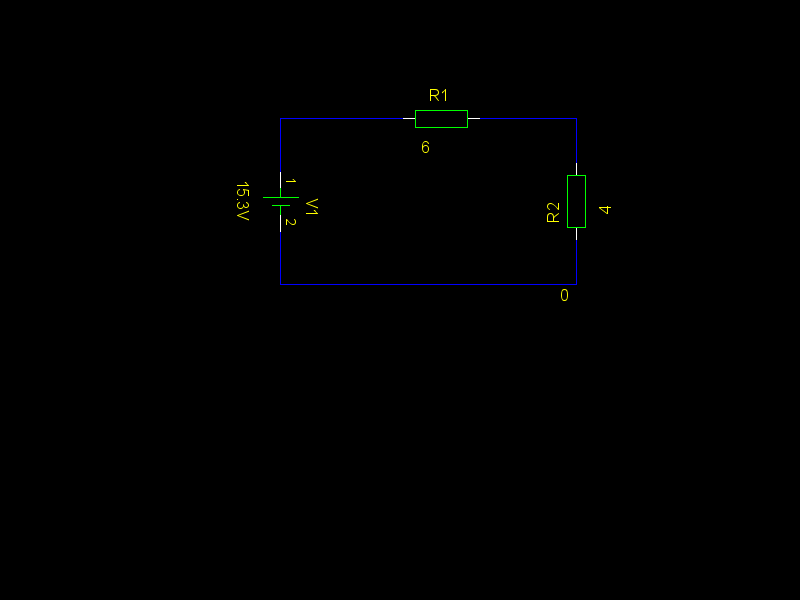
\includegraphics[width=9cm]{01.png}
\captionof{figure}{gschem shēma}
\label{att:1}
\end{figure}

\newpage
\subsection{darbs ar gnetlist}
\begin{verbatim}
    * Spice netlister for gnetlist
      R2 0 2 4
      R1 1 2 6
      V1 1 0 15.3V
     .END
\end{verbatim}
\subsection{darbs ar ngspice}

\begin{figure}[b!]
\centering
\begin{minipage}{.5\textwidth}
\centering
\includegraphics[width=6cm]{02.ps}
\captionof{figure}{Spriegums punktā 1 pret zemi}
\label{att:2}
\end{minipage}

\begin{minipage}{.5\textwidth}
\centering
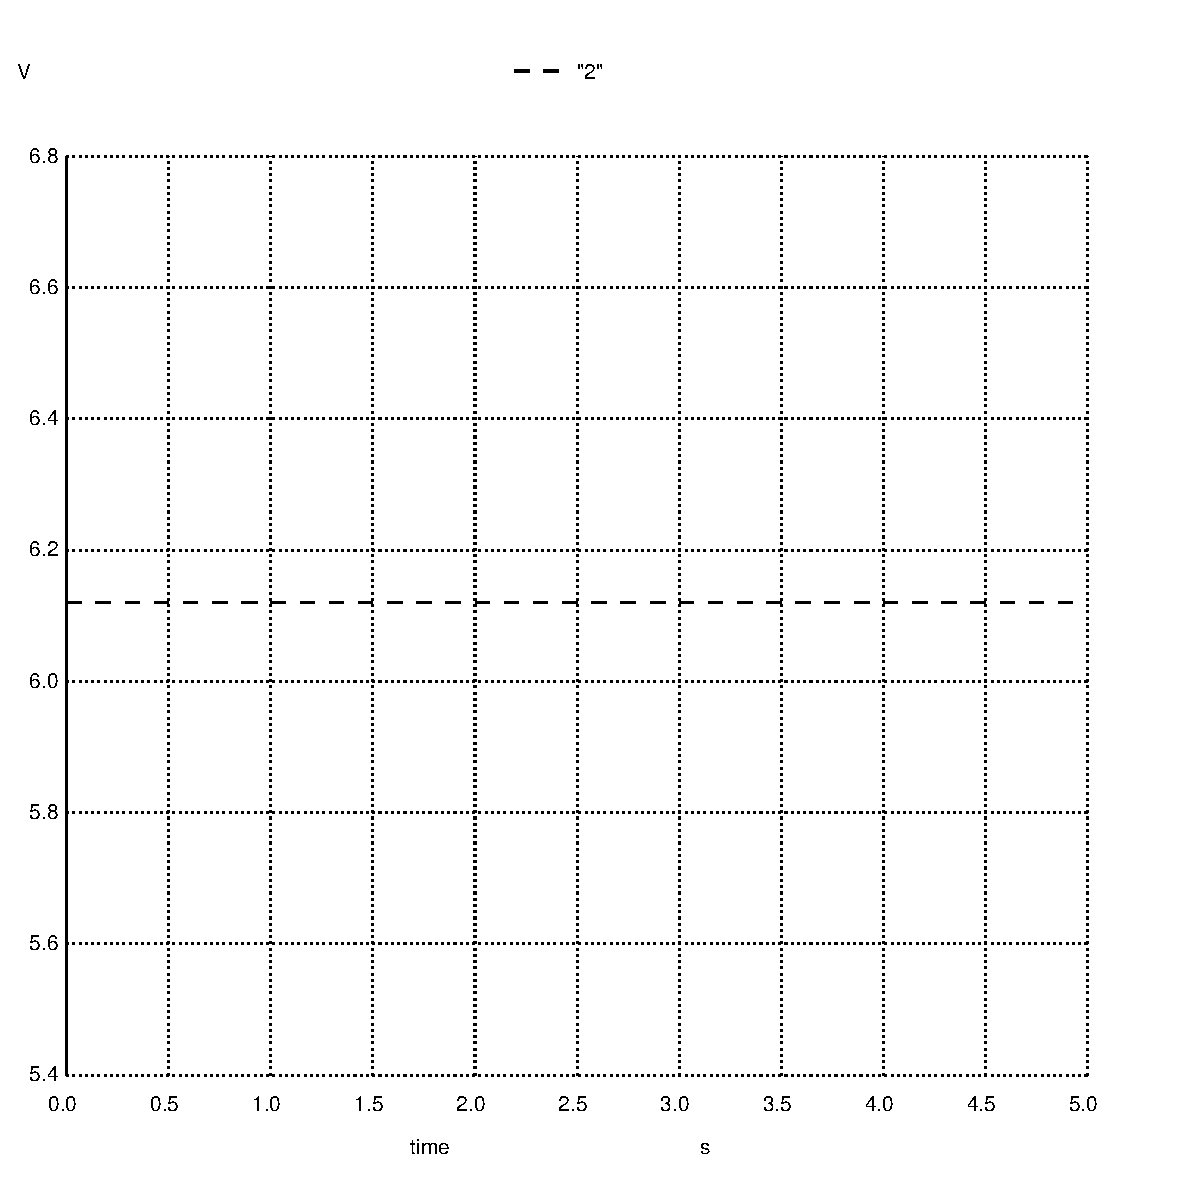
\includegraphics[width=6cm]{01.ps}
\captionof{figure}{Spriegums punktā 2 pret zemi}
\label{att:3}
\end{minipage}
\end{figure}

\newpage
\section{Darbs ar QUCS programmām}
Pēc sweep simulācijas (att. \ref{att:4}) var redzēt, ka mainoties R2 vērtībai no 5$ \Omega$ līdz 50$ \Omega$ spriegums izejas punktā palielinās (graf. \ref{att:5}). Jo lielāka R2 vērtība, jo lielāks izejas spriegums.


\begin{figure}[b!]
\centering
\rotatebox{270} {\includegraphics[width=\columnwidth]{1.2shema.ps}}
\captionof{figure}{}
\label{att:4}
\end{figure}

\begin{figure}[b!]
\centering
\rotatebox{-90}{\includegraphics[width=\columnwidth]{13.ps}}
\captionof{figure}{}
\label{att:5}
\end{figure}




\chapter{Secinājumi}
\begin{itemize}
\item Šajā laboratorijas darbā sāku apgūt shareLaTeX programmu, kā arī ar dažas citas simulācijas programām, kas ļoti palīdzēs arī citos priekšmetos, piemēram, kādos laboratorijas datbos;
\item Sāku apgūt LaTeX valodu;
\item Veicu pirmā laboratorijas darba atskaiti.
\end{itemize}

\begin{thebibliography}{1}
\bibitem{Oms}
Ohm's Law, Electrical Math and Voltage Drop Calculations (Revised Edition) by Tom Henry (December 1, 1992)
\bibitem{gschem}
 Goering, Richard (2004-12-13). "Do-it-yourselfer's EDA project wins open-source fans"
\end{thebibliography}

\end{document}
